\documentclass[10pt]{article}
\usepackage{polski}
\usepackage[left=1cm, right=1.5cm, top=0cm, bottom=1cm]{geometry}
\usepackage{multicol}
% \renewcommand{\familydefault}{\sfdefault}
\usepackage{lipsum}
\usepackage{graphicx}
\usepackage[T1]{fontenc}
\usepackage{charter}
\usepackage{enumitem}
\usepackage{fancyvrb}
\usepackage{nopageno}
\usepackage[dvipsnames]{xcolor}

\begin{document}

    % \hskip-1.55cm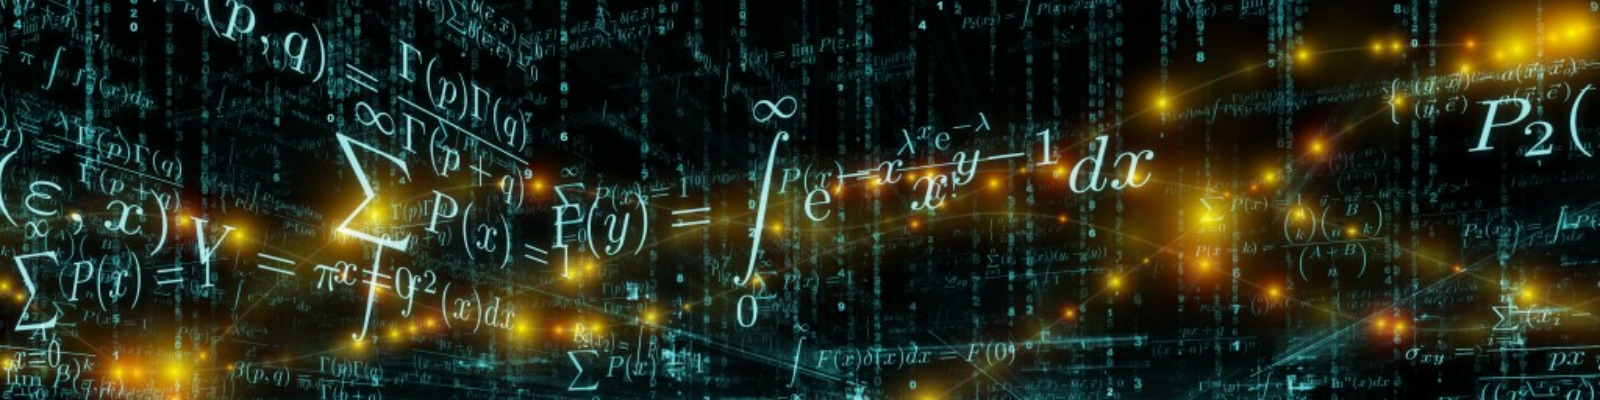
\includegraphics[scale=0.4]{banner.png}
    % \hskip-1.55cm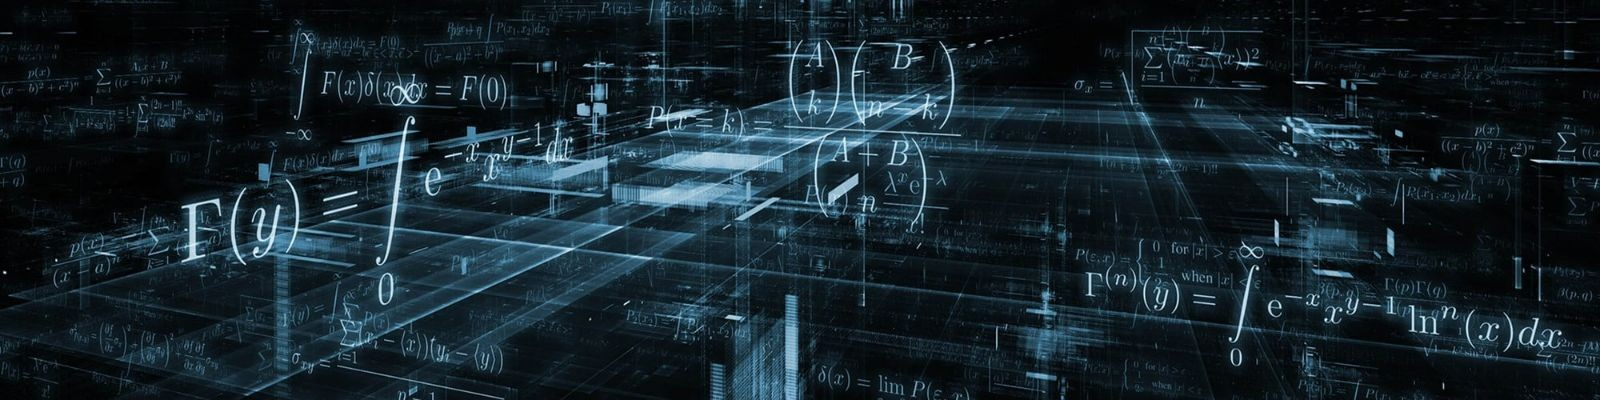
\includegraphics[scale=1.6]{banner4.jpg}
    \hskip-1.55cm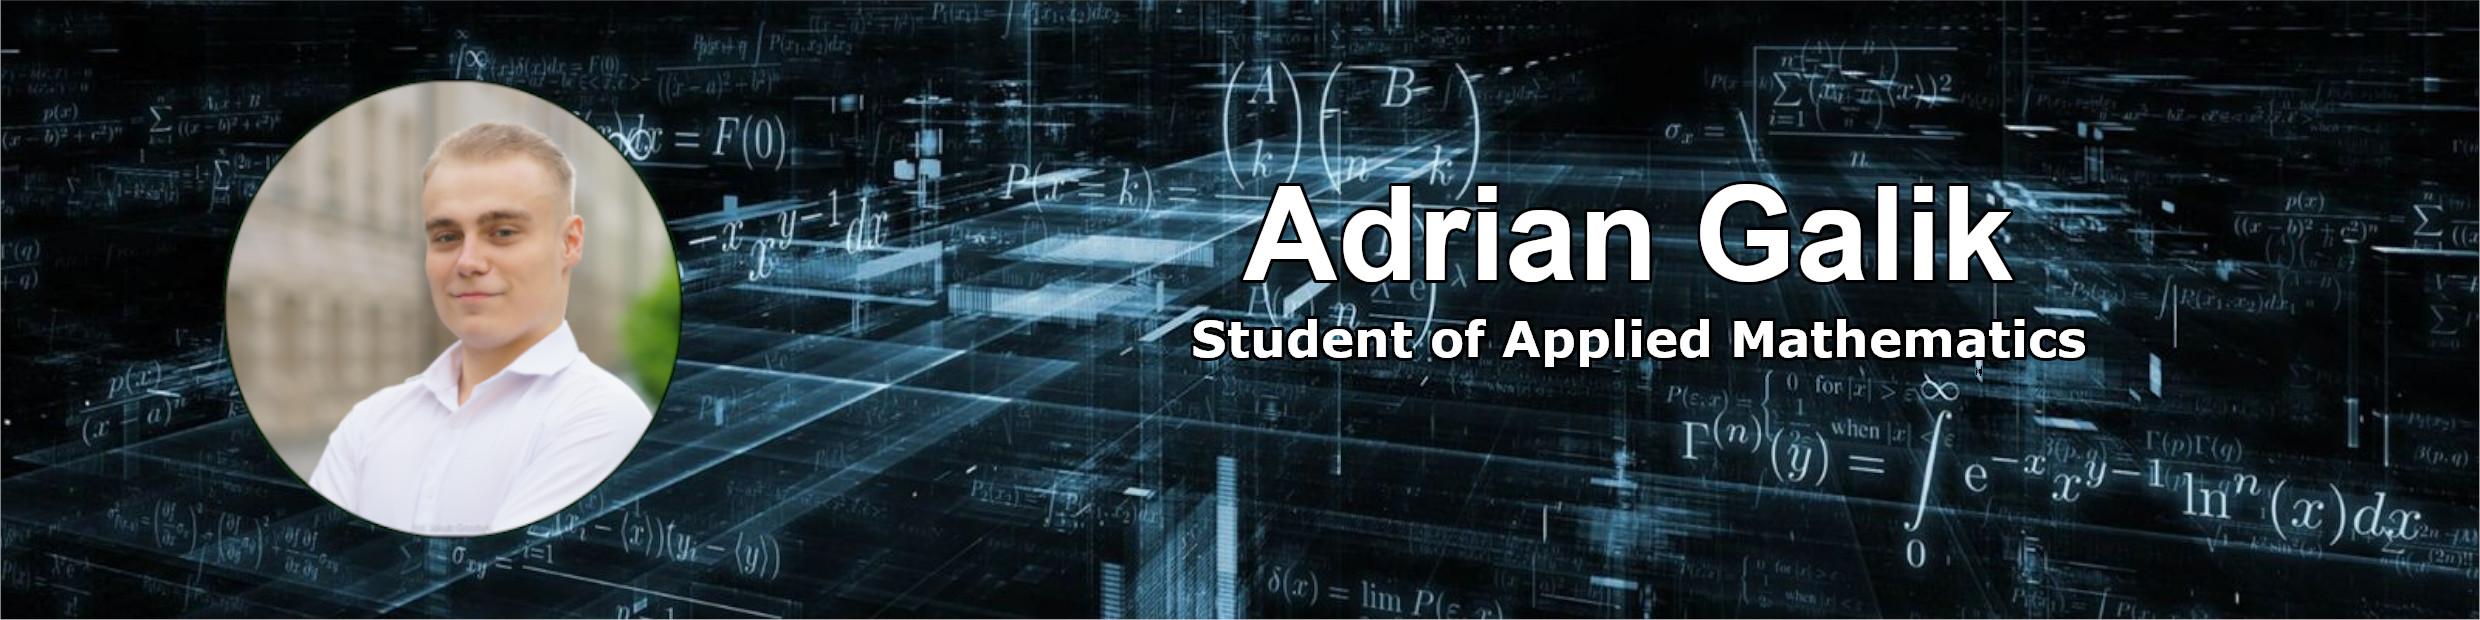
\includegraphics[scale=0.245]{benger_eng.jpg}
    % \hskip-1.55cm
\includegraphics[scale=1.6]{banner5.jpg}
    % \hskip-1.6cm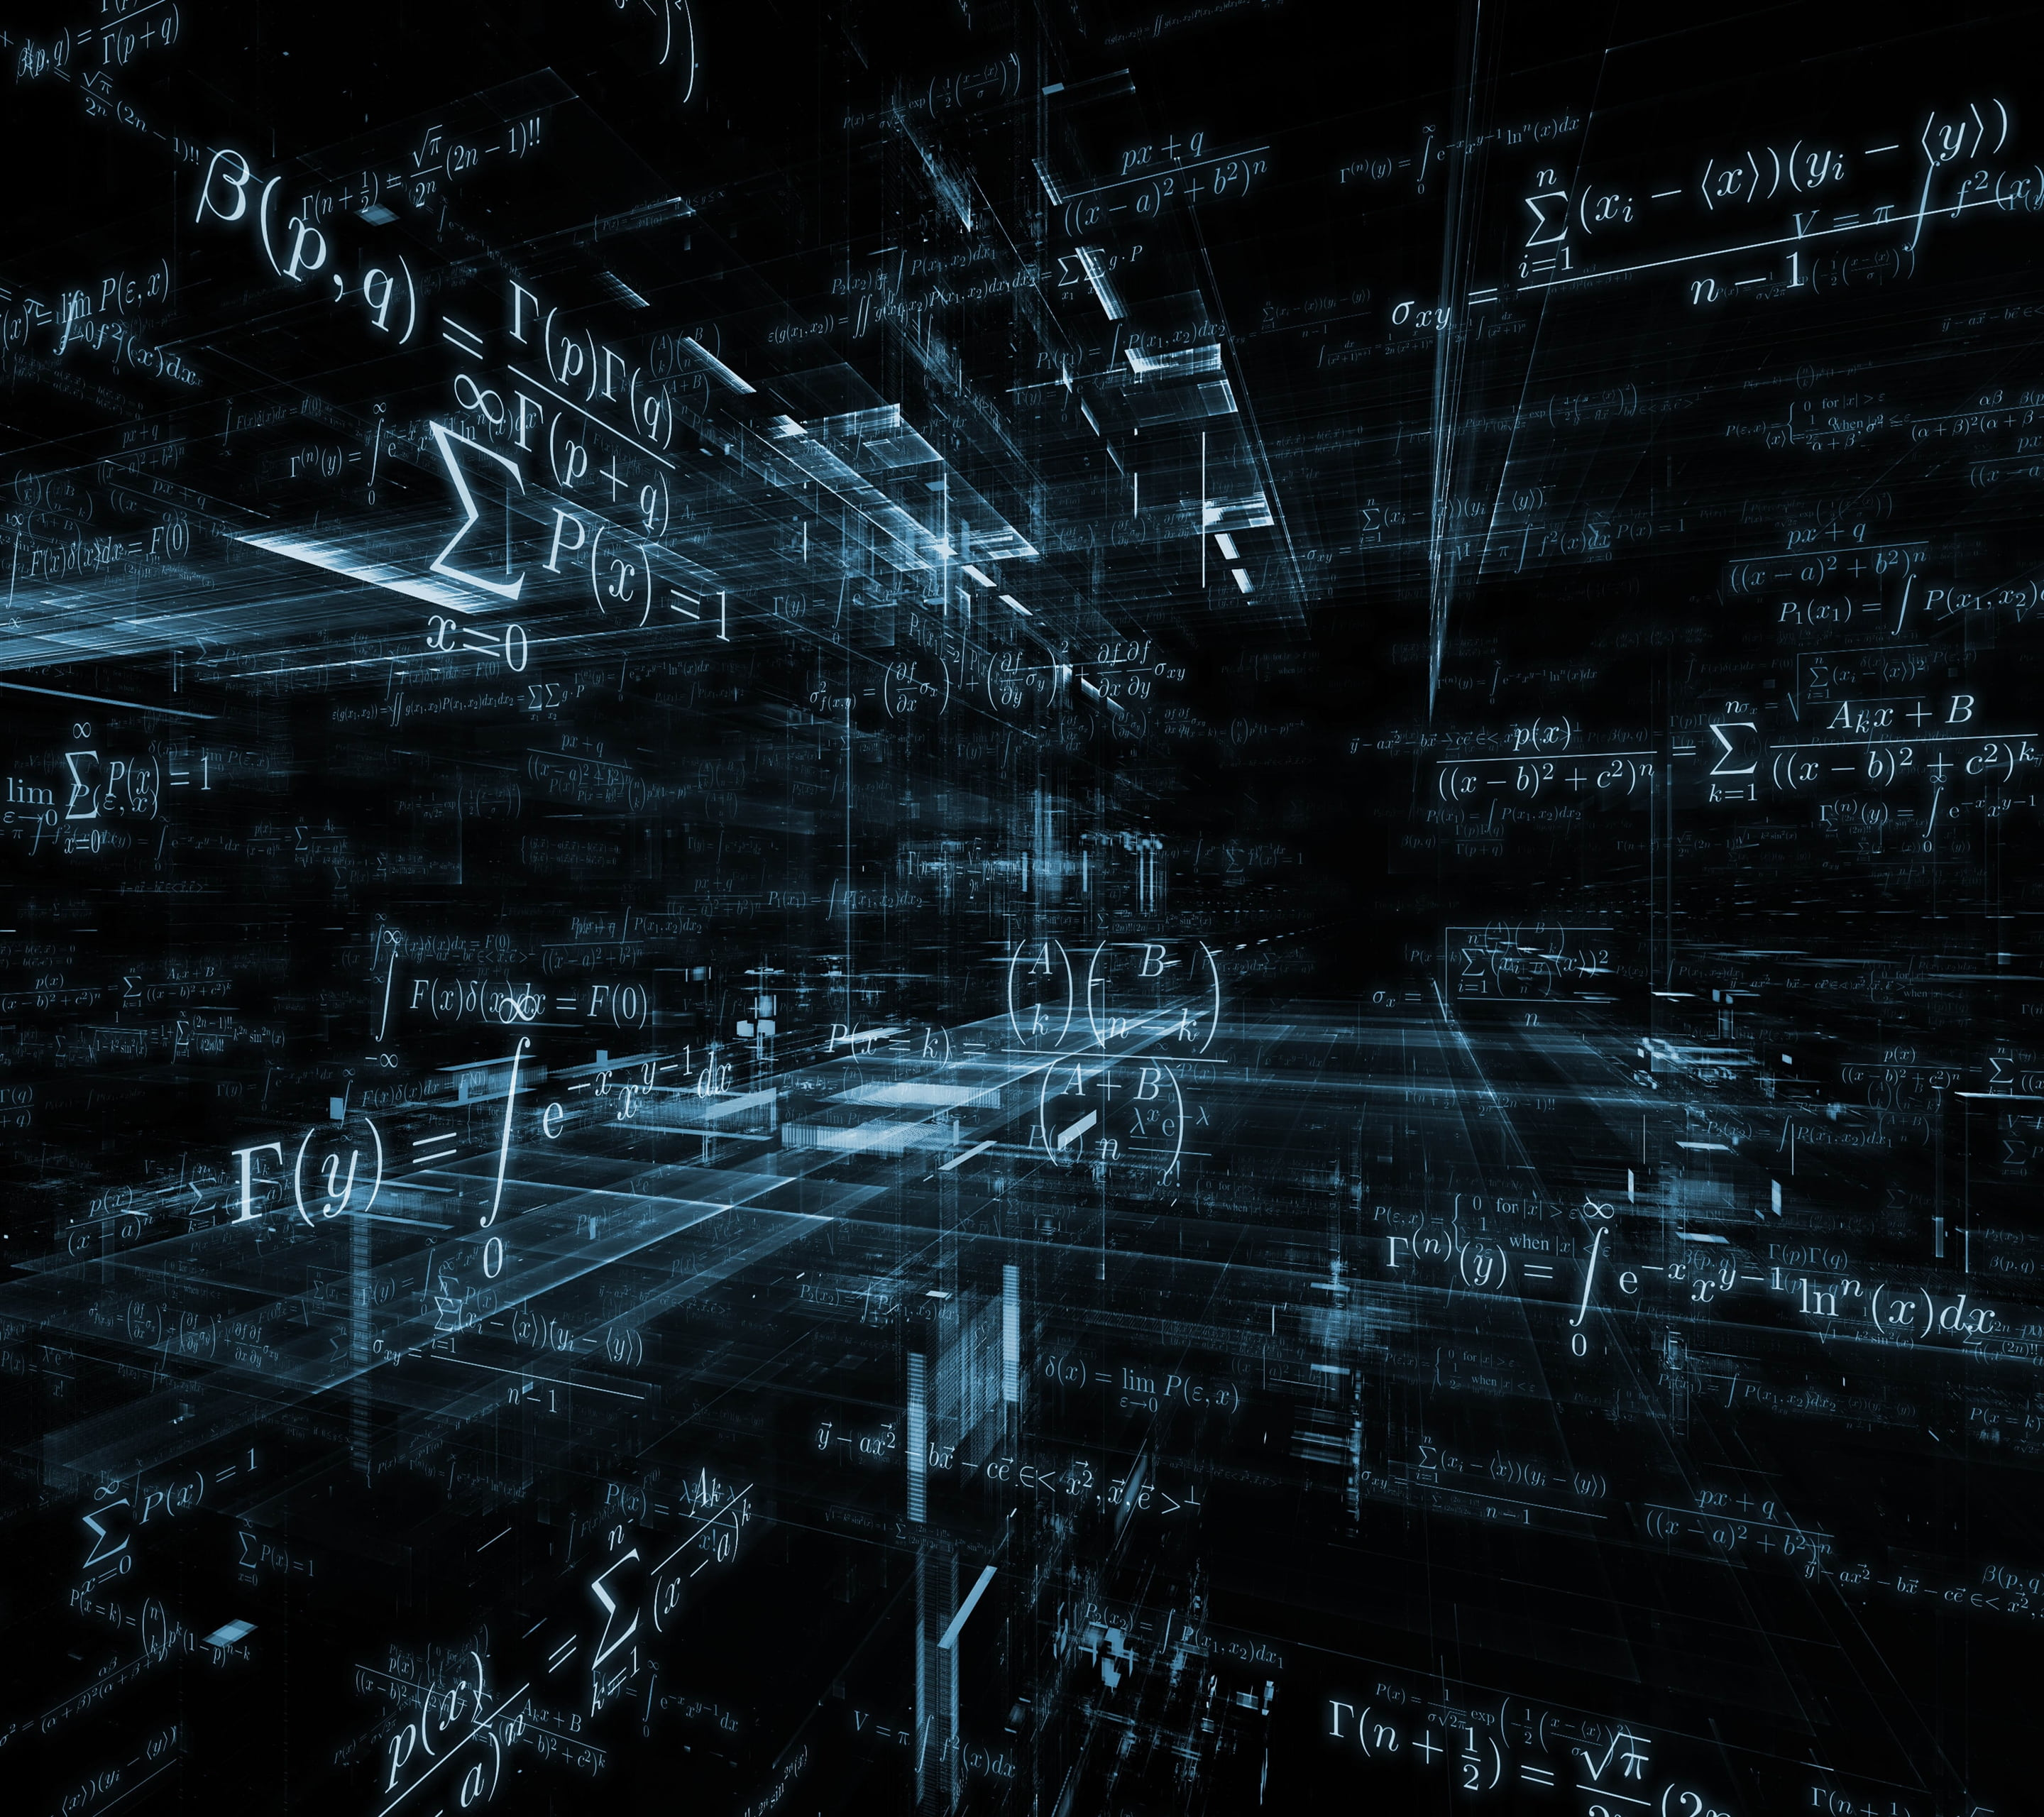
\includegraphics[height=0.20\textheight, width=1.5\textwidth]{banner2.jpg}
    % \hskip-1.6cm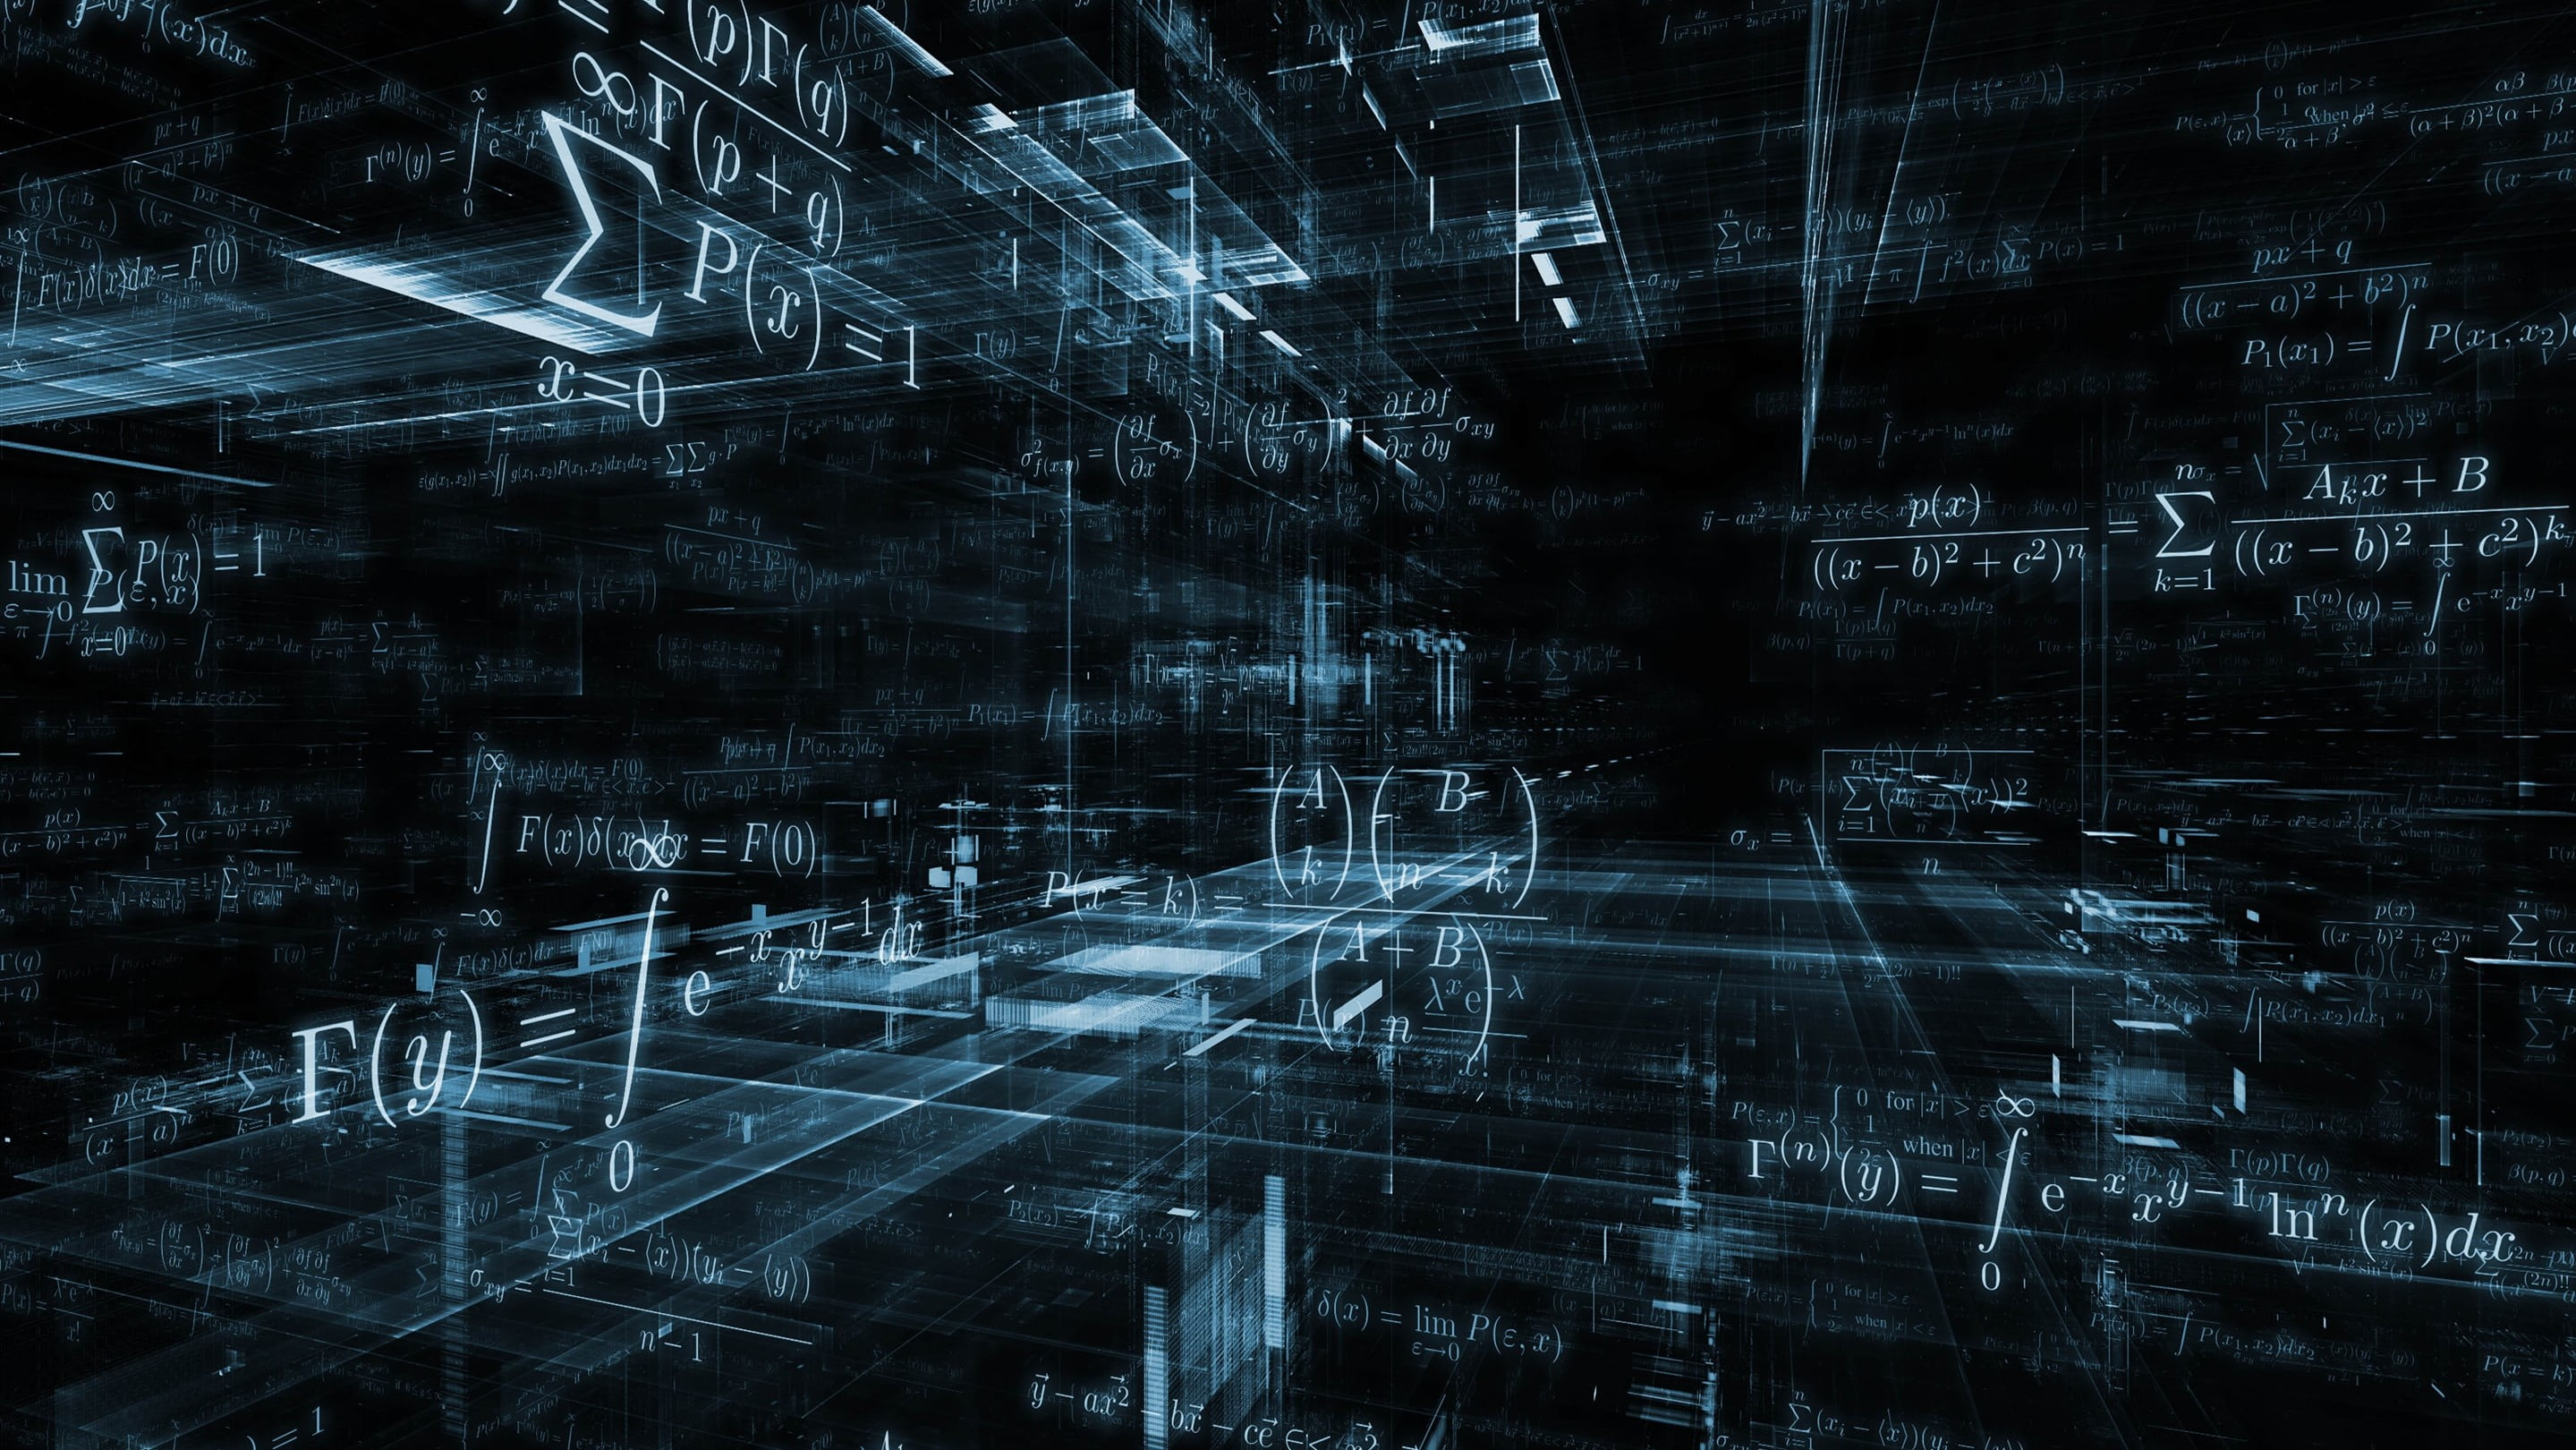
\includegraphics[height=0.25\textheight, width=1.5\textwidth]{banner3.jpg}
    \noindent
    \thispagestyle{empty}

    \vskip+0.4cm\begin{minipage}[t]{0.30\textwidth}
        \textbf{+48 663 383 000 \\
        adrian1galik@gmail.com \\
        github.com/Vexus1} \\ \\
        \rule{6cm}{1pt} \\ \\
        \fontsize{14pt}{14pt}{\textbf{\color{Violet}SKILLS:}}
        \fontsize{10pt}{10pt}
        \begin{itemize}[leftmargin=*]
            \setlength{\parskip}{0pt}
            % \setlength\itemsep{0pt} 
            \item \textbf{Python} intermediate level
            \item Programming libraries: \raggedright \\ \textbf{NumPy, Pandas, Pygame, OpenCV, TensorFlow, Keras} 
            \item Abstract data structures: \textbf{Stacks, Queues, Trees, Graphs}
            % \item Algorithmics
            \item Data base managing: \textbf{SQL}
            \item Mathematical models and \\ statistical methods \textbf{R language}
            \item Creating and managing of \\ websites: \textbf{HTML, CSS, JavaScript, React, Flask, PHP}
            % \item Applications of differential \\ equations
            \item Network projecting and managing
            \item Distributed version control: \textbf{Git}
            % \item Creating and managing of \\ websites: \textbf{HTML, CSS, JavaScript, Flask, PHP}
            % \item Text formatting language: \textbf{LaTeX}
            \item Operation system: \textbf{Linux}
            \item Numerical calculations: \textbf{Julia}
            \item Unix shell: \textbf{Bash} 
            \item Accelerated Container Application Development: \textbf{Docker}
            \item Analytical thinking
            \item Team work
        \end{itemize}
        \rule{6cm}{1pt} \\ \\
        \fontsize{14pt}{14pt}{\textbf{\color{Violet}LANGUAGES:}}
        \fontsize{10pt}{10pt}
        \begin{itemize}[leftmargin=*]
            \setlength{\parskip}{0pt}
            % \setlength\itemsep{0pt} 
            \item Polish native
            \item English C1
        \end{itemize}
        \rule{6cm}{1pt} \\ \\
        \fontsize{14pt}{14pt}{\textbf{\color{Violet}HOBBIES:}}
        \fontsize{10pt}{10pt}
        \begin{itemize}[leftmargin=*]
            \setlength{\parskip}{0pt}
            % \setlength\itemsep{0pt} 
            \item Machine learning
            \item Mathematics 
            \item Astrophysics
        \end{itemize}
    \end{minipage}
    \hfill % horizontal space between columns
    \begin{minipage}[t]{0.60\textwidth}
        \fontsize{14pt}{14pt}{\textbf{\color{Violet}ABOUT ME:}}
        \newline

        \fontsize{10pt}{10pt}
        Ambitious student of \textbf{Applayed Mathematics}. I'm using math 
         knowledge 
        to write algorithms related to \textbf{artificial intelligence},
        mainly \textbf{machine learning}.
        My favourite programing language is \textbf{Python} and I would like to use it in my work. In the future, I see myself in the field of \textbf{machine learning}. \\ \\
        \rule{11cm}{1pt} \\ \\
        \fontsize{14pt}{14pt}{\textbf{\color{Violet}EXPERIENCE:}}
        \fontsize{10pt}{10pt}
        \begin{itemize}[leftmargin=*]
            \setlength{\parskip}{0pt}
            % \setlength\itemsep{0pt} 
            % \item Internship in firm \textbf{Sports Media}. Network and computer systems 
            \item Science club \textbf{Robocik} operating at the Wrocław University of Technology.
            \textbf{Artificial intelligence} design, writing algorithms for pole detection
            by an autonomous underwater drone, which was prepared for the \textbf{TAC Challange}
            competition abroad. (\textbf{Python OpenCV})
            %  Preparation, development and validation of automated tests of
            % functionalities run during the preparation of the drone for swimming (\textbf{Python OpenCV})
            \item Programming projects in the \textbf{Python} language, i.e., a 2D game written
            in the object-oriented paradigm using the \textbf{Pygame} library
            numerical solution of Friedman's differential equation
            determining the evolution of the universe (\textbf{github})
            \item Internship in firm \textbf{Sports Media}. Computer networks and systems.
            \item Internship in firm \textbf{Zapaśnik IT}. Computer systems management
            \item Member of commite for Didactics and Student Rights
        \end{itemize}
        \rule{11cm}{1pt} \\ \\
        \fontsize{14pt}{14pt}{\textbf{\color{Violet}EDUCATION:}}
        \fontsize{10pt}{10pt}
        \begin{itemize}[leftmargin=*]
            \setlength{\parskip}{0pt}
            % \setlength\itemsep{0pt} 
            \item \textbf{Wrocław University of Science and Technology, Applied Mathematics, october 2021 - still}
            \item \textbf{Teleinformatics and Electronics School complex in Wrocław, \\ Technical school no. 7 (IT Technician), September 2017 - April 2021} 
        \end{itemize}
        \rule{11cm}{1pt} \\ \\
        \fontsize{14pt}{14pt}{\textbf{\color{Violet}CERTIFICATIONS:}}
        \fontsize{10pt}{10pt}
        \begin{itemize}[leftmargin=*]
            \setlength{\parskip}{0pt}
            % \setlength\itemsep{0pt} 
            \item \textbf{Qualification EE.09 - Programming, creating and administering \\ websites and databases}
            \item \textbf{Qualification EE.08 - Installation and operation of computer systems, peripherals and networks}
        \end{itemize}
        \rule{0pt}{0pt} \\ \\ \\ \\ \\ \\ \\ 
        \fontsize{7pt}{5pt}\selectfont  
        I hereby give consent for my personal data included in my application to be processed for 
        the purposes of the recruitment process under the European Parliament's and Council of the 
        European Union Regulation on the Protection of Natural Persons as of 27 April 2016, with 
        regard to the processing of personal data and on the free movement of such data, and repealing 
        Directive 95/46/EC.
    \end{minipage}

\end{document}